\documentclass[aspectratio=169]{beamer}
\usepackage{fancyvrb}
\usepackage{framed}
\usepackage{caption}
\usepackage{qrcode}
\usetheme{CambridgeUS}


\title{HEVM, a Smart Contract Verification Tool} 
\author{Mate Soos, Ethereum Foundation}
\date{25th of October 2023}
%\logo{sdfsdaf}


\begin{document}
\begin{frame}
    \titlepage 
\end{frame}

\begin{frame}{A bit about myself}
\begin{itemize}
\item PhD from INRIA Grenoble, France, wrote CryptoMiniSat, a SAT solver with the theory of Gauss-Jordan elimination
\item Worked in IT Security industry for 10+ years
\item Research at Kuldeep Meel's group for the past 5 years, mostly on counting and sampling
\item Working at Ethereum Foundation for the past 2 years
\end{itemize}
\bigskip

A lot of what I did were rewrite systems: preprocessors, inprocessors, etc. HEVM is in large part, a rewrite system

\end{frame}

% Outline frame
\begin{frame}{Outline}
    \tableofcontents
\end{frame}


% Lists frame

\section{Testing and the Ethereum Blockchain}
\begin{frame}{A Quick Recap of Testing}

\begin{columns}
\begin{column}{0.7\textwidth}
   Testing is a discipline. Reliable systems usually have a \textbf{testing strategy} encompassing at least parts of the test pyramid.
   
   As part of the tests, there are usually:
   \begin{enumerate}
   \item API specification that decribes what should happen, checked by 
   \textbf{positive tests}
   \item Bad outcomes that should not happen, usually checked by  \textbf{negative tests}
   \item A set of known bad states that should never be entered, checked by \textbf{invariant tests}
   \end{enumerate} 
\end{column}
\begin{column}{0.3\textwidth}  %%<--- here
    \begin{center}
     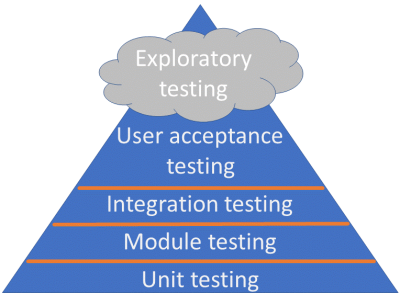
\includegraphics[scale=0.45]{triangle3.png}
     \end{center}
\end{column}
\end{columns}
\bigskip


Symbolic execution can help with finding ways to trigger \emph{all} negative tests and validate that invariants \emph{always} hold.

\end{frame}

\begin{frame}{A Quick Recap of Ethereum}
Ethereum is the second largest cryptocurrency in terms of value. Ethereum has:
\begin{itemize}
\item Stack-based VM, the Ethereum VM (EVM)
\item Contracts with code and storage
\item ACID execution semantics
\item EVM-specific programming language, Solidity and its IR, YUL
\item Proof-of-stake as its consensus layer
\item Soon a data availability layer ("proto-danksharding") for rollups
\end{itemize}

Downsides:
\begin{itemize}
\item Code and data are not clearly separated
\item JUMP destinations are known but dynamic jumps are possible
\item All EVM instructions operate on 256b values (!)
\end{itemize}

\end{frame}


\section{Symbolic Execution: A Recap}
\begin{frame}[fragile=singleslide]{Symbolic Execution -- straight line program}

Most execution works by running instructions concretely:
\begin{verbatim}
---             ax: 1   , bx: 2
mov %bx %ax     ax: 2   , bx: 2
add %ax $4      ax: 6   , bx: 2
\end{verbatim}
\bigskip

Symbolic execution, with symbolic state:
\begin{verbatim}
---             ax: v1  , bx: v2
mov %bx %ax     ax: v2  , bx: v2
add %ax $4      ax: v2+4, bx: v2
\end{verbatim}
\end{frame}

\begin{frame}[fragile=singleslide]{Symbolic Execution -- branching}
\begin{minipage}[t]{0.45\textwidth}
Concrete execution:
\begin{Verbatim}[fontsize=\small]
-----------     ax: 1    bx: 1
cmp %ax %bx     ax: 1    bx: 1
je .if_true     
; false
add %ax $4
jmp short .end
.if_true:
add %ax $5      ax: 6    bx: 1
.end:
\end{Verbatim}
\end{minipage}%
\begin{minipage}[t]{0.45\textwidth}
Symbolic execution, with symbolic state:
\begin{Verbatim}[fontsize=\small]
-----------     ax: v1   bx: v2
cmp %ax %bx     
je .if_true     
; false
add %ax $4      ax: v1+4 bx: v2
jmp short .end
.if_true:
add %ax $5      ax: v1+5 bx: v2
.end:
---- v1==v2 ->  ax: v1+5 bx: v2
---- v1!=v2 ->  ax: v1+4 bx: v2
\end{Verbatim}
\end{minipage}
\bigskip

For sybolic execution, we end up having to follow two executions. This can become exponential.

\end{frame}

\section{HEVM: An Overview}
\begin{frame}{HEVM}
\begin{itemize}
\item Uses the Ethereum Virtual Machine (EVM) for execution
\item Can do both concrete and symbolic execution
\item Takes as input negative/invariant test
\item Examines \emph{all}\footnote{loops/recursion is an issue, we have a loop/depth limit} execution paths from the starting state
\item Finds the set of requirements to reach all failing paths (i.e. \texttt{assert}-s)
\item Runs external tool (SMT solver) to find input to reach them
\item Displays call needed to trigger the bad state/invalidate the invariant
\end{itemize}
\end{frame}

%\begin{frame}[fragile=singleslide]{Symbolic Execution: example}
%Say your code looks like this:
%\begin{Verbatim}[frame=single, framerule=0.2mm, framesep=2mm,fontsize=\small]
%function overflow(uint a) public pure {
%	uint b;
%	unchecked { b = a + 1;}
%	assert(b > a);
%}
%\end{Verbatim}
%
%
%HEVM can find the case where $a=0xffffff\ldots$ to trigger the assert due to roll-around. HEVM gives you the \textbf{exact call to reproduce the bug}. This way of using HEVM can find a \emph{known-bad state}.
%
%\end{frame}

\begin{frame}[fragile=singleslide]{Symbolic Execution vs Fuzzing}
Say your code looks like this:

\begin{Verbatim}[frame=single, framerule=0.2mm, framesep=2mm,fontsize=\small]
function tricky(uint a, uint b) public pure {
	// solution: a = 10000983843024
	//           b = 9877982748934
	
	if (a * 2 + b == 29879950434982 &&
	    b / 2 == 4938991374467) {
		assert(false); // bad things happen
	}
}
\end{Verbatim}

Fuzzing never finds this edge-case. Symbolic execution always finds it.
\bigskip 

\textbf{In general, fuzzing is faster, but is incomplete. Symbolic execution is slower but complete.}

\end{frame}

\begin{frame}[fragile=singleslide]{Symbolic Execution: Invariant Checking}
You can describe \textbf{invariants} of your contract and write them as functions Then assert these functions every time the invariant must hold.
\begin{Verbatim}[frame=single, framerule=0.2mm, framesep=2mm,fontsize=\small]
function my_invariant() private pure returns inv {
	inv = ...calculate invariant...
}
	
function transfer(uint a) public pure {
	require(my_invariant());
	... your function code here ....
	assert(my_invariant());
}
\end{Verbatim}

Here, instead of a known-bad state, we validate that we are always in state that matches our expectations.
\end{frame}	


\begin{frame}[fragile=singleslide]{Symbolic Execution: Equivalence Checking}
You can ask HEVM to check whether two implementations are equivalent
\bigskip
\\

\begin{minipage}[b]{0.45\textwidth}
\begin{Verbatim}[frame=single, framerule=0.2mm, framesep=2mm,fontsize=\small]
function (...) public returns x {
  x = /known good computation/
      /uses lots of gas/
}
    \end{Verbatim}
  \end{minipage}
  \begin{minipage}[b]{0.45\textwidth}
  \begin{Verbatim}[frame=single, framerule=0.2mm, framesep=2mm,fontsize=\small]
function (...) public returns x {
  x = /complicated computation/
      /uses less gas/
}
\end{Verbatim}
\end{minipage}

HEVM can give you the exact \textbf{call to trigger the discrepancy} between the two functions. This way, you can safely improve the gas performance of your code.
\end{frame}

\section{HEVM: The Nitty-Gritty Details}
\begin{frame}{How HEVM works}
\centering
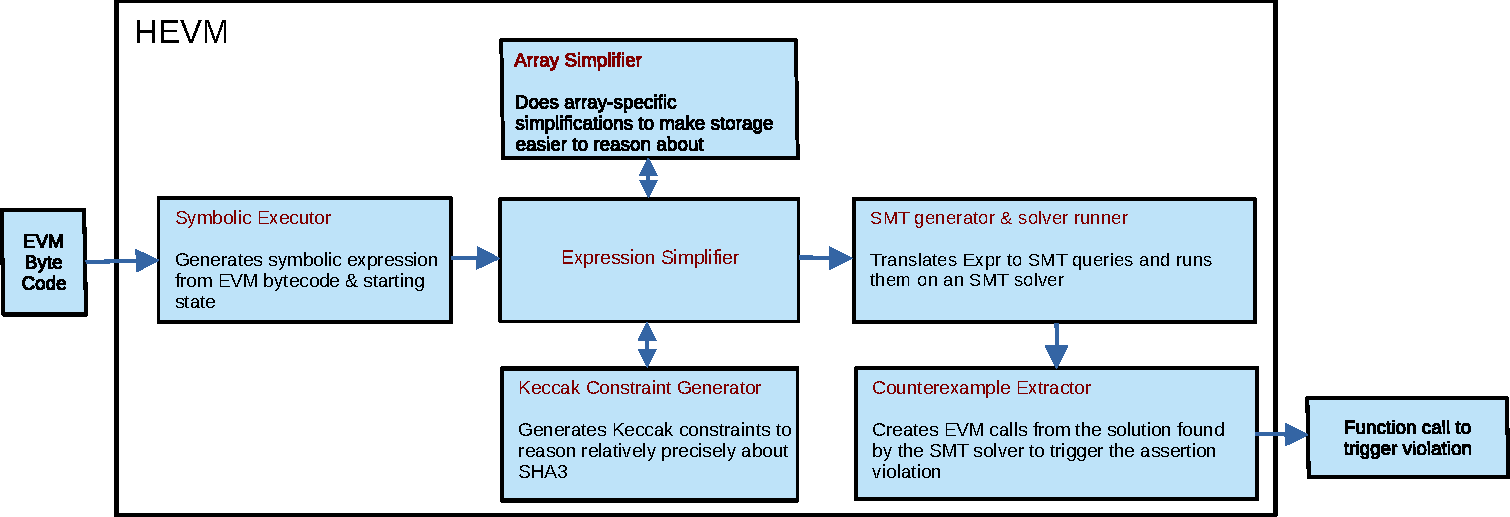
\includegraphics[scale=0.6]{HEVM-overview}

\end{frame}

\begin{frame}[fragile=singleslide]{Intermediate Representation}
\small

Through the interpreter we create the global expression that captures all end-states. We then take each end-state out and filter it for things we are looking for, e.g. assertion failures. This is our intermediate representation, similar to what YUL is for Solidity. Let's take the example:


\begin{Verbatim}[frame=single, framerule=0.2mm,framesep=2mm,fontsize=\small]
function overflow(uint a) public pure {
	uint b;
	unchecked { b = a + 1;}
	assert(b > a);
}
\end{Verbatim}

The expression to generate a counterexamle for this could look like:

\begin{Verbatim}[frame=single, framerule=0.2mm, framesep=2mm,fontsize=\small]
PLEq (Add (Var "a") (Lit 1)) (Var "a")
\end{Verbatim}

Notice: we use less-or-equal, because we want a \textbf{counterexample}
\end{frame}

\begin{frame}[fragile=singleslide]{Intermediate Representation: Writes}
When writing on top of a buffer, we represent it as:

\begin{Verbatim}[frame=single, framerule=0.2mm, framesep=2mm,fontsize=\small]
(ConcreteBuf "") // empty buffer
WriteWord (Lit 1) (Var "a") (ConcreteBuf "") //first write
WriteWord (Lit 2) (Var "b")  (WriteWord (Lit 1) (Var "a") (ConcreteBuf ""))
\end{Verbatim}
This can later be collapsed, e.g. in case the variables are concretized.
\bigskip

While this can be inefficient, it allows us perform symbolic execution as fast as possible, only reading/writing/transforming data at each instruction. We can (and do) later collapse \& simplify these writes.
\bigskip

NOTE: another way of doing this would be e.g. interval graphs
\end{frame}

\begin{frame}[fragile=singleslide]{Intermediate Representation: Keccak}
Keccak, i.e. SHA-3 is used extensively by all contracts in EVM. This is because e.g. storage of contracts is an \emph{unstructured array} of uint256. Hence, to implement e.g. maps and an arrays, one needs to use Keccak to map to a "random" position in storage, so as not to clash.
\bigskip

It's very expensive to accurately represent Keccak in SMT. Hence, we represent Keccak as an \emph{uninterpreted function} in SMT, with the following rules:
\begin{itemize}
\item We know the concrete value of the input $\rightarrow$ we add the axiom $keccak(input)=output$
\item Size of value hash differs $\rightarrow$ hash differs. We assert this for all pairs
\item Assert all pairs of keccak to be unequal if they don't match over \emph{partial} concrete values
\item Keccak value is never very small
\end{itemize}
\end{frame}

\begin{frame}[fragile=singleslide]{Intermediate Representation: Maps}
Storage of contracts is unstructured array of uint256. Solidity uses: $keccak (bytes32(key) || bytes32(id))$ to map $mymap[key]$ where $id$ is the map index:

\begin{Verbatim}[frame=single, framerule=0.2mm, framesep=2mm,fontsize=\small]
contract C {
    mapping(uint => uint) mymap_id0;
    mapping(uint => uint) mymap_id1;
}
\end{Verbatim}
We have solidity-specific rewrite rules to strip writes. So when writing two $keccak (bytes32(key) || bytes32(id))$-s on top of each other, and then reading, we traverse the list of writes to pick out the potentially matching one(s).
\bigskip

Notice that the SMT solver can use our Keccak rules to do this, too, but it's a lot slower
\end{frame}

\begin{frame}[fragile=singleslide]{Intermediate Representation: Simplification} 
We do all following rewrites to fixedpoint:
\begin{itemize}
\item Canonicalization of all commutative operators (concrete value first)
\item Canocicalization of all less-than/greater-than/etc operators
\item Canonicalization of all Keccak expressions to match Solidity patterns
\item Stripping writes when they are not read
\item Stripping reads when they are not used
\item Constant folding
\item (In)equality propagation
\item All meaningful rewrites, such as min/max/add+sub/add+add/sub+sub/etc.
\item Delayed simplification of Keccak expressions to keep structure as much as possible
\end{itemize}
\end{frame}

\begin{frame}[fragile=singleslide]{Intermediate Representation: Haskell to the Rescue}

Haskell supports algebraic data types (ADTs), so our intermediate representation can fully typed. Furthermore, Haskell supports pattern matching, so we rewrite rules are easy to read \& write:
\begin{Verbatim}[frame=single, framerule=0.2mm, framesep=2mm,fontsize=\small]
    -- syntactic Eq reduction
    go (Eq (Lit a) (Lit b))
      | a == b = Lit 1
      | otherwise = Lit 0
    go (Eq (Lit 0) (Sub a b)) = eq a b
    go (Eq a b)
      | a == b = Lit 1
      | otherwise = eq a b
\end{Verbatim}
\end{frame}

\begin{frame}[fragile=singleslide]{What can we use the IR for?}
\begin{itemize}
\item Finding counterexamples with SMT solvers
\item Constant extraction: helping other fuzzers with "magic numbers"
\item Subsitute constants and fold: we can build a fuzzer
\item Not just failing branches: automated test-case generation
\end{itemize}

\end{frame}

\begin{frame}[fragile=singleslide]{Solving the IR: Creating a Fuzzer}

Fuzzing sounds strange given that HEVM is a symbolic execution engine. However:
\begin{itemize}
\item The IR is actually a very clean representation of the problem at hand
\item Due to the extensive simplifications applied, it can contain specific constants that may be very hard to find otherwise
\item IR \emph{could} be transpiled to assembly (potentially through \texttt{C}), and executed as a program
\end{itemize}
\bigskip

Notice that geth, the normal EVM concrete executor is incredibly slow. Hence a transpiled IR could achivee serious speedup.

\end{frame}

\begin{frame}[fragile=singleslide]{Solving the IR: using an SMT Solver}
The IR is translated in a straightforward manner to SMT. Let's say the expression is:

\begin{Verbatim}[frame=single, framerule=0.2mm, framesep=2mm,fontsize=\footnotesize]
PLEq (Add (Var "a") (Lit 1)) (Var "a")
\end{Verbatim}
\bigskip

The SMT expression for this could be:

\begin{Verbatim}[frame=single, framerule=0.2mm, framesep=2mm,fontsize=\footnotesize]
(set-logic QF_AUFBV)
(define-sort Word () (_ BitVec 256))
(declare-const varA (Word))
(assert (bvule (bvadd varA (_ bv1 256)) varA))
(check-sat)
\end{Verbatim}

Z3 gives the answer:

\begin{Verbatim}[frame=single, framerule=0.2mm, framesep=2mm,fontsize=\footnotesize]
sat
(
  (define-fun varA () (_ BitVec 256)
    #xffffffffffffffffffffffffffffffffffffffffffffffffffffffffffffffff)
)
\end{Verbatim}
\end{frame}

\begin{frame}[fragile=singleslide]{Using HEVM}

Install foundry [1]. Get static HEVM binary [2]. Install z3 [3]. Add foundry test cases, and prepend with \texttt{``prove\_''} the ones you want HEVM to use:

\begin{Verbatim}[frame=single, framerule=0.2mm, framesep=2mm,fontsize=\footnotesize]
function prove_add(uint x, uint y) public pure {
    unchecked { if (x + y < x) return; }
    assert(x + y >= x);
}
\end{Verbatim}

Then run with:

\begin{Verbatim}[frame=single, framerule=0.2mm, framesep=2mm,fontsize=\footnotesize]
forge build
hevm test
\end{Verbatim}


\bigskip

[1] \url{https://github.com/foundry-rs/foundry}

[2] \url{https://github.com/ethereum/hevm/releases}

[3] \url{https://github.com/Z3Prover/z3}
\end{frame}


\begin{frame}[fragile=singleslide]{Benchmarking}
\small
To test and improve the performance of HEVM, we use a benchmark repository [1]. Here, you can test your example problem against other full-featured symbolic execution engine Halmos [2]:

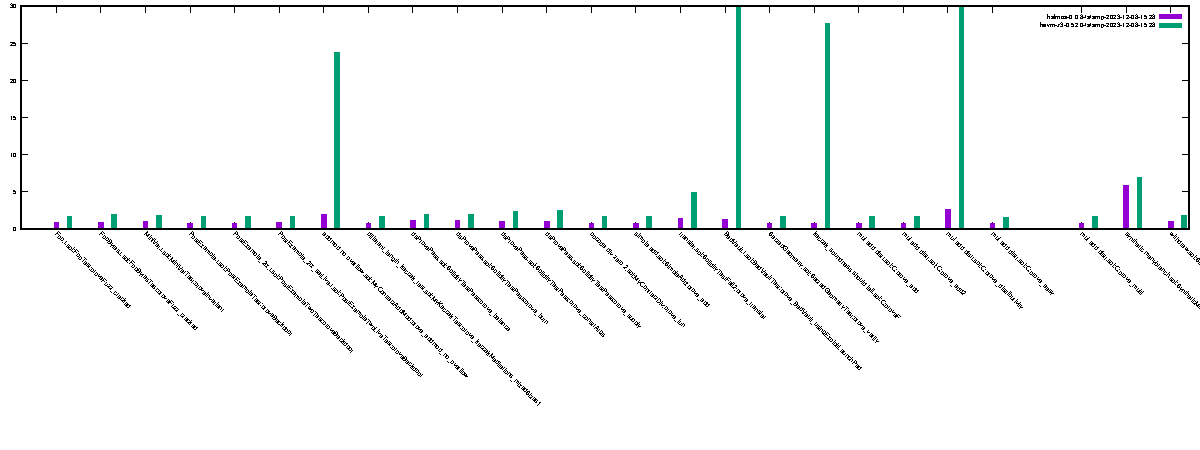
\includegraphics[scale=0.7]{boxchart}

\bigskip
[1] \url{https://github.com/eth-sc-comp/benchmarks/}

[2] \url{https://github.com/a16z/halmos}
\end{frame}


%\begin{frame}[fragile=singleslide]{Contributing Back to HEVM}
%
%The HEVM repository uses \texttt{nix} for ease of development:
%
%
%
%You now have a full development environment, with all necessary tools installed, including Z3.
%\bigskip 
%
%HEVM is written in Haskell, but there are many areas that can be contributed to without deep knowledge of Haskell. For example, expression simplification:
%
%\begin{Verbatim}[frame=single, framerule=0.2mm, framesep=2mm,fontsize=\footnotesize]
%    go (Add a b)
%      | b == (Lit 0) = a
%      | a == (Lit 0) = b
%      | otherwise = add a b
%\end{Verbatim}
%\end{frame}

\begin{frame}[fragile=singleslide]{Limitations}
HEVM has a number of inherent limitations:

\begin{itemize}
\item Loops are challenging. The option \texttt{--max-iterations N} raises the iteration limit until which loops are examined.
\item Recursion, and parametric calls can cause HEVM to only partially explore the state
\item Complicated mathematical expressions (e.g. division, modulo) can cause a challenge
\item HEVM itself is not verified, and neither are the SMT solvers. Some SMT solvers will in be able to emit a proof, though
\end{itemize}
\end{frame}

\section{Conclusions}
\begin{frame}[fragile=singleslide]{Conclusions}

HEVM is a fully-featured, easy-to-use tool that can help find bugs in EVM bytecode. It is fully-featured, with a robust internal representation (IR) that can significantly lower the burden on the SMT solvers used. It is tailored to the EVM system by having Keccak- and array/map-specific rewrites to lower the complexity of the final SMT expression.
\bigskip

Download HEVM from \url{https://github.com/ethereum/hevm/releases}
\bigskip
%\qrcode{https://github.com/ethereum/hevm/releases}

Development environment is easy to set up:
\begin{Verbatim}[frame=single, framerule=0.2mm, framesep=2mm,fontsize=\footnotesize]
sh <(curl -L https://nixos.org/nix/install) --daemon
git clone https://github.com/ethereum/hevm/
nix-shell
cabal repl test
[...]
> :main
\end{Verbatim}

\end{frame}



\end{document}
